\titleformat{\chapter}
{\normalfont\fontsize{12}{15}\centering}{Anexos \thechapter.}{0.3em}{}[]

\clearpage
\thispagestyle{empty}
\begin{center}
  \vspace*{\fill}
  \phantomsection
  Apéndices
  \addcontentsline{toc}{chapter}{Anexos}
  \vspace*{\fill}
\end{center}
\clearpage

\appendix
\uextra{Apendice}{Dispositivo Raspberry Pi 4 Model B}
\begin{figure}[h!]
  \centering
  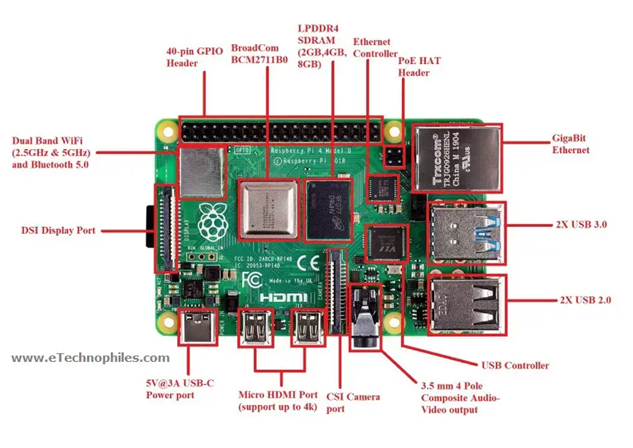
\includegraphics[width=0.95\textwidth]{Anexos/1.arquitectura-raspberry.png}
  \caption{Arquitectura del Raspberry Pi 4 Model B}
  \label{fig:raspberry-architecture}
\end{figure}

\uextra{Apendice}{ Validación del sistema de monitoreo acústico}

{\small
      \begin{longtable}[c]{c p{3.5cm} p{2.2cm} p{2.2cm} p{3.5cm}}
            \hline
            \textbf{Requerimiento} & \textbf{Descripción}                                                                                    & \textbf{Entrada}                                                 & \textbf{Salida}                                                       & \textbf{Análisis}                                                                                                                                  \\
            \hline
            \endfirsthead

            \hline
            \textbf{Requerimiento} & \textbf{Descripción}                                                                                    & \textbf{Entrada}                                                 & \textbf{Salida}                                                       & \textbf{Análisis}                                                                                                                                  \\
            \hline
            \endhead
            \endfoot
            \endlastfoot

            R1                     & Captura continua del audio ambiental a través de micrófonos.                                            & Señales de audio del entorno a través del hardware del micrófono & Eventos discretos etiquedados del audio.                                     & Verificación de que el sistema de hardware y software es capaz de procesar el audio de forma constante sin interrupciones.                         \\
            \addlinespace
            R2                     & Procesamiento del audio para clasificarlo en eventos sonoros predefinidos.                              & Flujo de datos de audio                                          & Clasificación del sonido (ej. voz, silencio, golpe).                  & Evaluación de los modelos de IA como YAMNet y Vosk para clasificar audio.                                                  \\
            \addlinespace
            R3                     & El sistema aprende y mantiene un perfil de la actividad acústica ``normal'' del entorno.                & Conjunto de de datos de audio clasificado con contexto temporal                & Existe o no una anomalia& Verificación de que el sistema puede detectar o no las anomalias                                           \\
            \addlinespace
            R4                     & Comparación de la actividad en tiempo real con el perfil de normalidad para detectar patrones anómalos. & Secuencia de eventos en tiempo real             & Identificación de una anomalía o evento atípico.                      & Pruebas para validar que modelos como Isolation Forest y LSTM Autoencoder pueden detectar correctamente las desviaciones del perfil de normalidad. \\
            \addlinespace
            R5                     & El sistema realiza una consulta verbal al usuario al detectar una anomalía.                             & Detección de una anomalía                                        & Emisión de una pregunta de voz pregrabada (ej. ``¿Está todo bien?''). & Verificación de que la consulta de voz se activa de forma automática y es clara para el usuario.                                                   \\
            \addlinespace
            R6                     & Permitir al usuario responder para cancelar una emergencia.                                             & Respuesta de voz del usuario (ej. ``Estoy bien'').               & El sistema cancela la alerta.                                         & Pruebas de funcionamiento para confirmar que el sistema puede procesar la respuesta del usuario y detener la activación de la alerta.              \\
            \addlinespace
            R7                     & El sistema envía notificaciones de emergencia si la anomalía es crítica o el usuario no responde.       & Falta de respuesta del usuario o gravedad de la anomalía         & Envío de notificaciones.                                              & Pruebas de integración para garantizar que las notificaciones se envían de forma automática y rápida.                                              \\
            \bottomrule
            \addlinespace

            \caption{Requerimientos del sistema acústico}
            \label{tab:requerimientos_sistema_acustico}
      \end{longtable}
}

